\documentclass{../source/Experiment}

\major{信息工程}
\name{姚桂涛}
\title{华为云鲲鹏BigData Pro集群搭建
}
\stuid{3190105597}
\college{信息与电子工程学院}
\date{\today}
\lab{-}
\course{数据分析与算法设计}
\instructor{赵明敏}
\grades{}
\expname{华为云鲲鹏BigData Pro集群搭建
}
\exptype{-}
\partner{}
\begin{document}
    \makecover
    \makeheader

    \section{实验介绍与目的}
        实验基于华为云OBS和华为云ECS服务构建一个存算分离的基本架构,并通过运行一个计算程序来完成存算分离架构的验证。
        
        实验的实验数据存储在OBS中,通过在ECS上部署开源组件(Hadoop和Spark)构成计算环境,最后编写Spark程序访问存储在OBS上的数据进行计算。

        计算验证的例子是统计数据中单词的出现频次,并输出结果。

    \section{华为云环境准备}
        \subsection{购买华为云ECS}
        弹性云服务器 ECS(Elastic Cloud Server)是一种可随时自助获取、可弹性伸缩的云服务器,帮助用户打造可靠、安全、灵活、高效的应用环境,确保服务持久稳定运行,提升运维效率。


        选择云服务器ECS,可以轻松构建具有以下优势的计算资源:
        \begin{itemize}
            \item 无需自建机房,无需采购以及配置硬件设施。
            \item 分钟级交付,快速部署,缩短应用上线周期。
            \item 快速接入部署在全球范围内的数据中心和边界网关协议BGP(Border Gateway Protocol)机房。
            \item 成本透明,按需使用,支持根据业务波动随时扩展和释放资源。
            \item 提供GPU和FPGA等异构计算服务器、弹性裸金属服务器以及通用的x86架构服务器。
            \item 支持通过内网访问其他阿里云服务,形成丰富的行业解决方案,降低公网流量成本。
            \item 提供虚拟防火墙、角色权限控制、内网隔离、防病毒攻击及流量监控等多重安全方案。
            \item 提供性能监控框架和主动运维体系。
            \item 提供行业通用标准API,提高易用性和适用性。
        \end{itemize}

        主要流程为:购买ECS,配置安全组规则。

        做好这些之后就可以通过远程工具进行连接了。

        \subsection{购买华为云OBS}

        对象存储服务OBS(Object Storage Service,OBS)可以提供海量、安全、高可靠、低成本的数据存储能力,可供用户存储任意类型和大小的数据。适合企业备份/归档、视频点播、视频监控等多种数据存储场景。

        可以应用于大数据分析,OBS提供的大数据解决方案主要面向海量数据存储分析、历史数据明细查询、海量行为日志分析和公共事务分析统计等场景,向用户提供低成本、高性能、不断业务、无需扩容的解决方案。

        主要流程为:购买OBS,记录IPv4地址。

        \subsection{掌握AK/SK的获取}
        
        访问密钥(Access Key ID/Secret Access Key,简称AK/SK)包含访问密钥ID(AK)和秘密访问密钥(SK)两部分,是华为云的长期身份凭证,可以通过访问密钥对华为云API的请求进行签名。

        华为云通过AK识别访问用户的身份,通过SK对请求数据进行签名验证,用于确保请求的机密性、完整性和请求者身份的正确性。

        掌握AK/SK后,做好记录,在后面配置OBS调用接口的时候,需要使用AK/SK进行签名验证。

    \section{Hadoop集群搭建}
        Hadoop是一个由Apache基金会所开发的分布式系统基础架构。用户可以在不了解分布式底层细节的情况下,开发分布式程序。充分利用集群的威力进行高速运算和存储。Hadoop实现了一个分布式文件系统( Distributed File System),其中一个组件是HDFS(Hadoop Distributed File System)。HDFS有高容错性的特点,并且设计用来部署在低廉的(low-cost)硬件上;而且它提供高吞吐量(high throughput)来访问应用程序的数据,适合那些有着超大数据集(large data set)的应用程序。HDFS放宽了(relax)POSIX的要求,可以以流的形式访问(streaming access)文件系统中的数据。

        主要流程为:通过PuTTY远程登录并配置ECS,获取JDK的安装路径,搭建Hadoop伪分布式集群,将Hadoop与OBS互联。

    \section{Spark集群搭建与验证存算分离}
        Spark 是使用 scala 实现的基于内存计算的大数据开源集群计算环境.提供了 java,scala, python,R 等语言的调用接口。

        本实验中使用Spark读取OBS数据,并使用Python编写Spark程序。

        搭建好Spark后,为了支持Python语言,可以安装Pyspark工具,然后就可以编写pyhton程序,对OBS中上传的数据进行处理了。
        \begin{figure}[H]
            \centering
            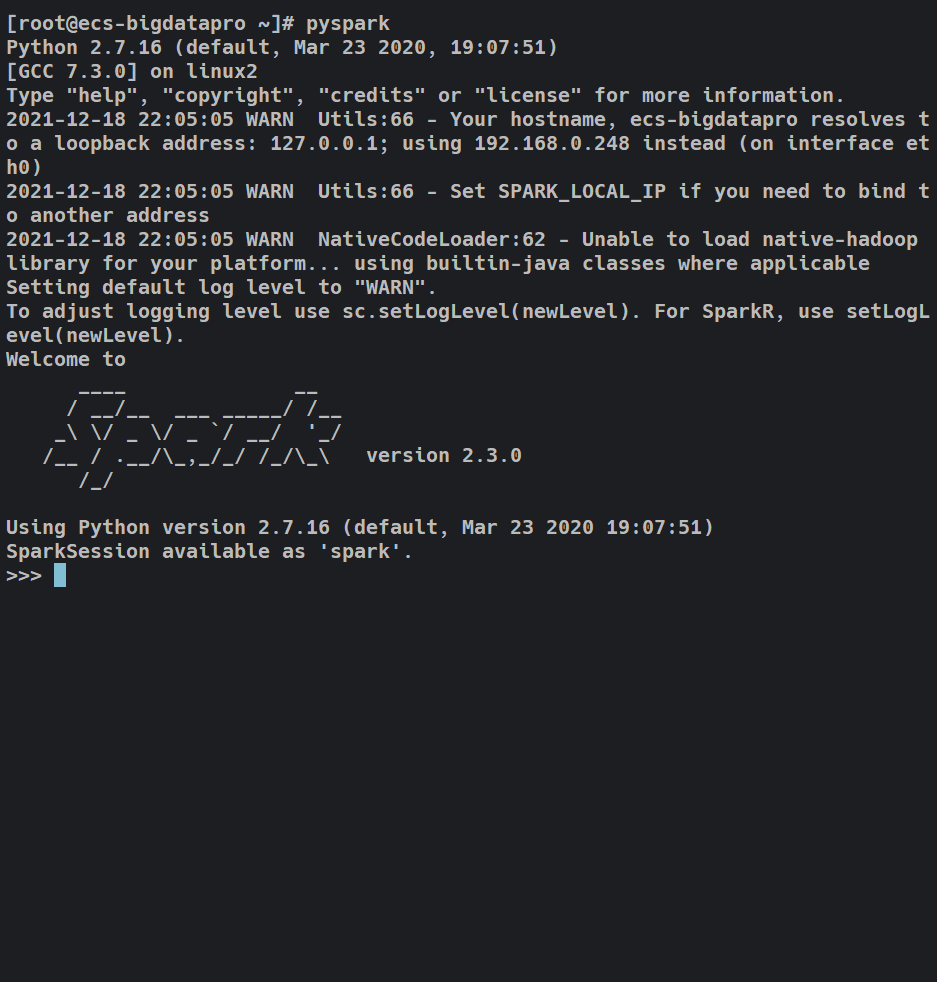
\includegraphics[width = 0.8\textwidth]{spark}
            \caption{启动pyspark}
        \end{figure}

        \begin{figure}[H]
            \centering
            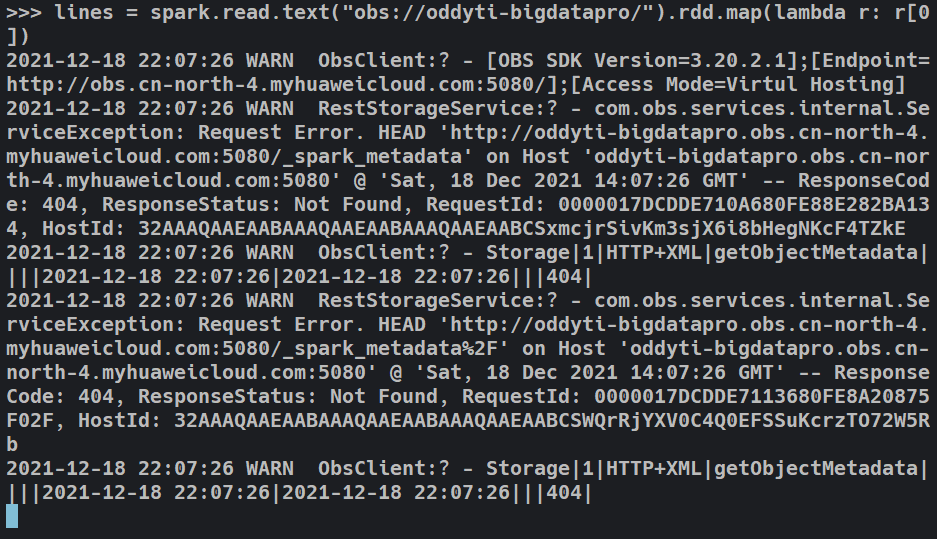
\includegraphics[width = 0.8\textwidth]{obs}
            \caption{读取OBS桶的内容}
        \end{figure}

        \begin{figure}[H]
            \centering
            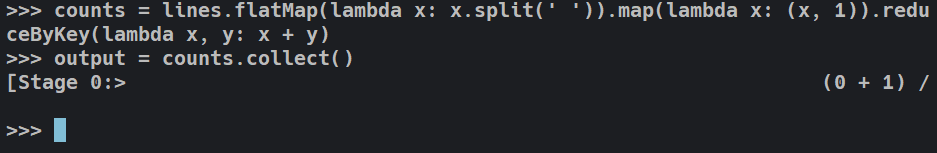
\includegraphics[width = 0.8\textwidth]{code}
            \caption{存算分离代码}
        \end{figure}

        \begin{figure}[H]
            \centering
            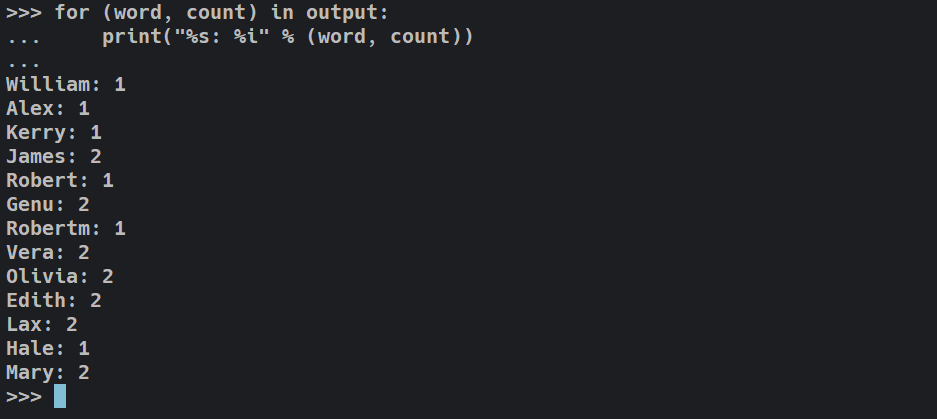
\includegraphics[width = 0.8\textwidth]{resault}
            \caption{存算分离结果}
        \end{figure}
    \section{释放华为云服务}
        做完实验后,需要释放我们购买的ECS与OBS。

\end{document}